%!TEX root = Slic3r-Manual.tex

Il ya deux façons d'organiser les param\`etres de configuration: exporter et importer les param\`etres de configuration, et des profils. Le premier est disponible en mode simple et expert, alors que les profils sont disponibles uniquement en mode expert.

\section{Export et Import de la Configuration} % (fold)
\label{sub:exporting_and_importing_configuration}
\index{configuration!export}
\index{configuration!import}

L'ensemble actuel d'options de configuration peut \^etre tout simplement export\'e via le menu File (Fichier)  \texttt{Export Config}. Cela permet se sauvegarder toutes les valeurs dans un fichier texte avec l'extention \texttt{.ini} .  Les fichiers pr\'ec\'edemment enregistr\'es peuvent \^etre charg\'es avec le menu File (Fichier) \texttt{Load Config} (charger la configuration).

Cela donne un des moyens rudimentaires pour stocker des param\`etres de configuration pour les diff\'erents besoins. Par exemple, un ensemble avec des vitesses d'impression l\'eg\`erement plus rapides, ou un motif de remplissage diff\'erent. Cependant, cette façon d'organiser les choses va vite devenir frustrante, car chaque changement mineur d'un param\`etre pourrait \^etre \`a dupliqu\'e dans de nombreuses configurations. Pour cette raison, les profils sont de façon plus appropri\'ee de g\'erer plusieurs configurations.

Cette m\'ethode permet \'egalement le transfert de configurations entre machines, ou le stockage \`a distance.

% section exporting_and_importing_configuration (end)


\section{Profils} % (fold)
\label{sec:profiles}
\index{profiles}
\index{profils}

Apr\`es quelques impressions, il deviendra \'evident qu'il est utile d'avoir un ensemble d'options de configuration \`a choisir, et que certains param\`etres changent plus souvent que d'autres. En mode expert, des profils peuvent \^etre cr\'e\'es pour les param\`etres d'impression, de Filament et d'imprimante, dans l'espoir que les param\`etres d'imprimante changent peu souvent, de filaments rarement, cependant les param\`etres d'impression peuvent \^etre modifi\'es pour chaque mod\`ele. Ces diff\'erents profils peuvent \^etre m\'elang\'es et combin\'es \`a volont\'e, et peuvent \^etre s\'electionn\'es dans leurs onglets respectifs, ou directement \`a partir de la surface de travail.

\subsection{Cr\'eation des Profils} % (fold)
\label{sub:creating_profiles}
\index{profiles!create}
\index{profils!cr\'eation}

Ouvrez l'onglet souhait\'e et modifiez les param\`etres si n\'ecessaire. Une fois satisfait, cliquez sur l'ic\^one de sauvegarde vers la gauche au-dessus des titres de r\'eglage, et donner un nom appropri\'e \`a l'invite.

\begin{figure}[H]
\centering
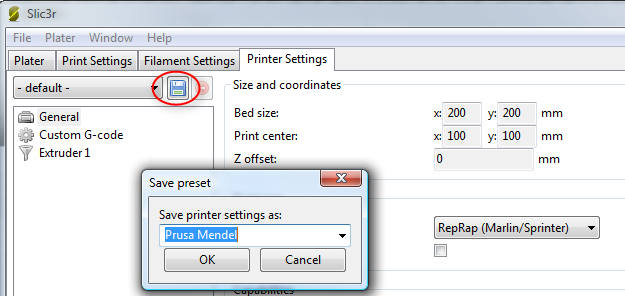
\includegraphics[keepaspectratio=true,width=1\textwidth]{organising/creating_a_profile.png}
\caption{Sauver un profil.}
\label{fig:creating_a_profile}
\end{figure}

\index{profiles!delete}
\index{profils!effacer}
Les profils peuvent \^etre supprim\'es, en choisissant le profil \`a supprimer et en cliquant sur le bouton rouge supprimer \`a c\^ot\'e du bouton Enregistrer.

\begin{figure}[H]
\centering
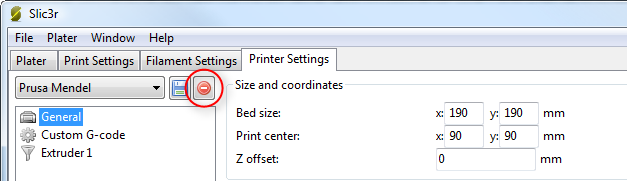
\includegraphics[keepaspectratio=true,width=1\textwidth]{organising/deleting_a_profile.png}
\caption{Effacer un profil.}
\label{fig:deleting_a_profile}
\end{figure}

% subsection creating_profiles (end)


% section profiles (end)